% ===== AAAI-27 spine draft: Experiments (merged) =====
\section{Experiments}\label{sec:experiments}

\subsection{Experimental Setup}\label{sec:setup}

We evaluate on \model{}, a 60-block DiT editor, on edit batteries
spanning five categories -- color, background, style, removal, and
addition -- over natural photographs and one flat-art source (10 cases
for the time-lens saturation sweep and the preview lever, 20 for the
IoU-based onset and CFG-truncation checks); every quantitative number
is paired with a per-image visual verdict recorded before the
aggregate is read, per the predict-look-gate protocol above. Three
readouts do the reporting: the frozen output head's decode, scored
zero-shot with CLIP against a small label bank; cross-seed probes,
including a 48-seed fixed-prompt outcome probe whose independent unit
is one generation; and, for the tuned lens, held-out $R^2$ against the true
conditional-pass velocity. Two further checkpoints sharing \model{}'s
transformer classes -- FireRed-Image-Edit-1.1, an independent
fine-tune, and Rapid-AIO, a 4-step distilled merge -- let us ask
whether a finding persists beyond one training run
(tested below).
Statistical units follow the claim: explicit-prompt patch probes are basis
diagnostics, whereas fixed-prompt tests contribute one mean-pooled vector per
generation. Their $p$-values use fold-matched label permutations; held-out
selection uses exact Poisson-binomial inference (Boogu) or exact within-group
rank tests (Qwen).

\subsection{The Realized Edit Is Predictable Early}\label{sec:early}

\noindent\textbf{Question.} Does the edit unfold gradually, or is the
final outcome readable before the frozen head agrees?

\paragraph{In time.} If the edit surfaced progressively, the readout would
saturate late and at roughly the same rate. Running the time lens over a battery of
10 cases across 5 edit categories, the step at which $P(\text{target})$
first reaches within $0.05$ of its final value is instead
\emph{edit-dependent} and mostly \emph{immediate}: color, background, and
style edits reach the criterion at step 0--2, and only a wholesale
new-object insertion (\emph{add\_boat}) does so as late as step 7. A finer
IoU-mask-based onset measurement over 20 cases shows the split is
categorical, not continuous: 18 of 20 -- spanning final-edit-area
fraction $0.003$ to $0.99$ -- onset at step 0 regardless of how large or
novel-looking the finished edit is, and no continuous proxy predicts the
delay (edge-novelty $\rho{=}0.24$, $p{=}0.30$; area $\rho{=}{-}0.44$,
running the \emph{wrong} way). Only the two edits that insert genuinely
novel structure with no existing pixels to build on -- \emph{add\_boat}
and \emph{add\_runner} -- start late.

\paragraph{In depth, the naive lens says ``late''.} The frozen depth lens
tells a different-looking story. Decoding \emph{car\_red}'s intermediate
layers through the model's own head, the edit becomes head-readable only
in a sharp snap between layers 48 and 54 of 60 -- exactly the familiar
mid-stack ``nothing happens yet'' appearance of an LLM logit lens.

\paragraph{But the realized outcome is predictable 40 layers earlier.}
An explicit-prompt probe first reveals the basis mismatch: predicting
which of three colors was requested reaches $0.883$ patch-token accuracy at
\textbf{layer 6}, step 4, where the frozen head reads only
$P(\text{red car}){=}0.111$ (Figure~\ref{fig:mechanism}). To separate
outcome prediction from reading a color word, we hold both source and
the underspecified prompt ``change the car to a different color'' fixed
across 48 new seeds and label each final image post hoc. One mean-pooled
vector per generation predicts the realized color at L6/step 4 with
$0.667$ balanced accuracy (chance $0.333$; $p{=}0.002$). Thus the outcome,
not merely the instruction, is linearly predictable early; this does not
claim irreversible commitment.

\begin{figure}[t]
  \centering
  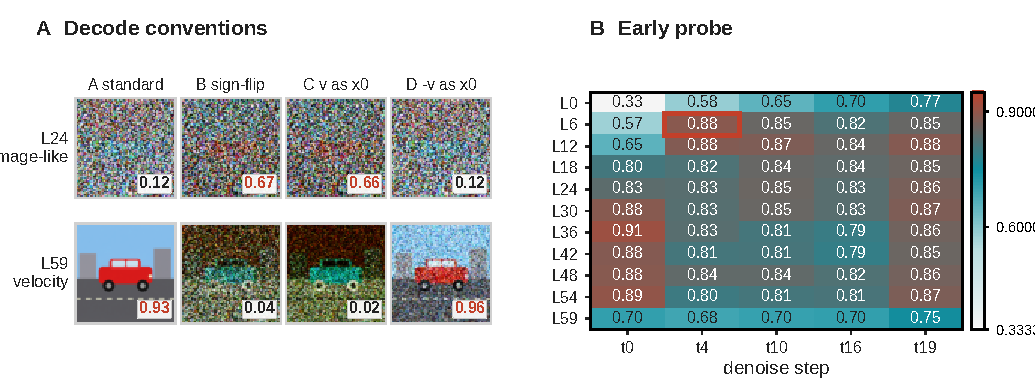
\includegraphics[width=\columnwidth]{figs/fig5_mechanism/fig5_mechanism.pdf}
  \caption{\textbf{Decode convention flips; the probe reads early.}
  \textbf{A}: four \emph{car\_red} decodes reverse convention between L24
  and L59. \textbf{B}: a requested-color basis diagnostic reaches $0.883$
  patch-token accuracy at L6/$t$4 while the frozen head still reads noise
  (chance $0.33$). Patches are not independent experimental units; the
  generation-level fixed-prompt result is $0.667$ over 48 generations.}
  \label{fig:mechanism}
\end{figure}

\paragraph{Prediction generalizes and supports selection.}
Table~\ref{tab:early} summarizes continuous-hue replications and held-out
best-of-five tests. Natural-photo mug and tree edits replicate while the
heterochromatic-eyes task is null ($p{=}0.796$); the independent 40-block
Boogu editor also carries an early hue readout, although its terminal layer
is stronger. Selection succeeds on Boogu and two Qwen target tasks. Actual
interrupted captures plus winner reruns save about 68\% versus full
best-of-five, but only select the closest available candidate.

\begin{table}[t]
\caption{Early prediction and held-out selection. Q/B denote Qwen/Boogu;
parentheses give chance or random-selection baselines.}
\label{tab:early}
\centering
\footnotesize
\setlength{\tabcolsep}{2.1pt}
\begin{tabular}{@{}lllll@{}}
\toprule
Setting & Readout & Metric & Result & Evidence \\
\midrule
Car fixed & Q L6/$t$4 & Bal. acc.$\uparrow$ & .667 (.333) & $p{=}.002$ \\
Car hue & Q L6/$t$2 & MAE$\downarrow$ & $22.3{\to}8.3^\circ$ & $R^2{=}.815$ \\
Tree hue & Q L6 & MAE$\downarrow$ & $55.9{\to}11.4^\circ$ & $p{=}.005$ \\
Mug hue & Q L6 & MAE$\downarrow$ & $17.0{\to}10.7^\circ$ & $p{=}.005$ \\
Boogu hue & B L4/$t$2 & MAE$\downarrow$ & $39.9{\to}6.9^\circ$ & $p{=}.005$ \\
Boogu select & B L4 best-5 & Success$\uparrow$ & 8/12 (20\%) & $p{=}4.1{\times}10^{-5}$ \\
Tree select & Q L6/$t$2 & MAE$\downarrow$ & $95.2{\to}46.5^\circ$ & $p{=}3.7{\times}10^{-7}$ \\
Car select & Q best-5 & MAE$\downarrow$ & $25.7{\to}11.1^\circ$ & $p{=}.0086$ \\
\bottomrule
\end{tabular}
\end{table}

\paragraph{Where the instruction enters.} A complementary text-stream
ablation locates where the prompt is \emph{consumed}: zeroing the model's
text tokens in only the first 11 blocks garbles the whole scene, while
zeroing them after layer 36 barely dents the edit ($P(\text{red}){=}0.993$).
The instruction is fused into the image stream early; for this color edit,
later text tokens are dispensable by layer 36 -- the ``injection'' stage of the circuit in
Figure~\ref{fig:teaser}, whose full text-band table is in the supplement.
Together with the probe, this gives the paper's five-stage picture:
injection ($\le$L36), early outcome prediction, a target-image code, translation
(L52--54), and the output head.
\noindent\textbf{Takeaway.} Time onset is mostly immediate; the frozen depth
lens looks late, but generation-level probes read the realized outcome from L6.

\subsection{The Edit Is Translated Late: Two Codes}\label{sec:translate}

\noindent\textbf{Question.} If probes read the outcome early, what mid-stack
code is converted at L52--54? Three measurements answer this: at an intermediate layer
the frozen head yields a per-token vector $v_\ell$ we normally treat as a
velocity, forming $\hat x_0 = x_t - \sigma_t v_\ell$ (variant A). Decoding
$v_\ell$ instead \emph{directly}, as if it were already a clean latent
(variant C), inverts the story: for \emph{car\_red} at step 4, at L24 the
standard decode A scores $P(\text{red}){=}0.12$ (still wrong-colored)
while the direct decode C already scores $0.66$; at L59 this reverses (A
$=0.93$, C $=0.02$). The mid-stack is not blank -- it encodes the target
content in an \emph{image-like} convention, and a narrow band near the top
reconciles it to the velocity convention the head consumes. (This is a
whole-vector reweighting, not a literal sign flip: essentially no
individual channel of $v_\ell$ has a negative slope against $v_{59}$, mean
$0.003$.)

\paragraph{The conversion location is stable; its width is timestep-dependent.} A dense
every-layer sweep from L44 to L59 (Figure~\ref{fig:boundary}) locates the
A/C crossover precisely: transition midpoint L53.6 at step 16 (width one
layer) and L52.7 at step 4 (width four layers). The midpoints differ by
under one layer, so the boundary's \emph{location} is stable across these
timesteps even though its sharpness is not. Crucially, the
cross-seed probe accuracy is close to \emph{flat} ($0.77$--$0.84$) across
every layer from L44 through L58 and drops only at the terminal layer L59
($0.68$--$0.70$). So the translation that changes what the head can read
(L52--54) and the loss of linear separability (L59) are two \emph{distinct}
events sharing a neighborhood: the target-image code survives the
translation intact and is degraded only by the final, velocity-specific
projection. Coarse family sweeps place measurable style and background
crossovers in the same terminal band; removal and addition remain
inconclusive because their between-variant CLIP margins are too small.

\begin{figure}[t]
  \centering
  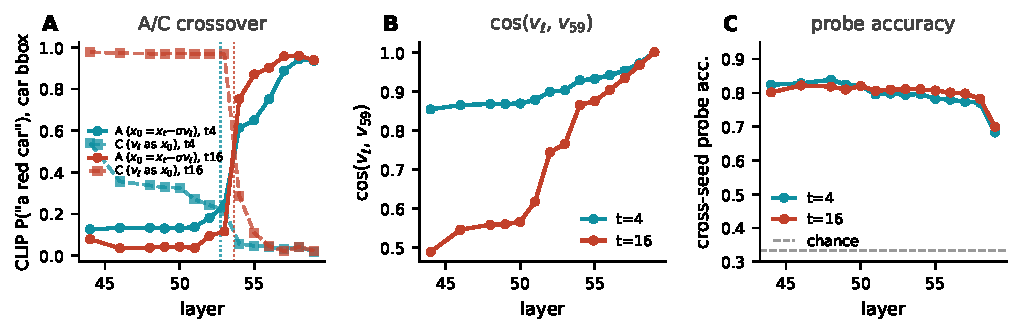
\includegraphics[width=\columnwidth]{figs/fig10_boundary/fig10_boundary.pdf}
  \caption{\textbf{Translation near L52--54.} Dense L44--L59 sweep on
  \emph{car\_red}. \textbf{A--B}: the decode-crossover midpoint changes by
  under one layer between $t{=}4,16$, while transition width changes from
  four layers to one. \textbf{C}: probe accuracy stays flat through L58 and
  drops only at L59.}
  \label{fig:boundary}
\end{figure}

\paragraph{A tuned lens renders the image-like code, layer by layer.} To
test whether the mid-stack code is image-like rather than a probe
artifact, we fit a per-(layer, timestep) tuned lens, as described
above, on exactly three source images -- one each from
\emph{remove}/\emph{background}/\emph{addition} -- and evaluate the entire
\emph{car\_red} source and color family \emph{zero-shot}. Held-out $R^2$
rises with depth from $0.73$--$0.89$ at L6 to
$0.998$ at L59, whose frozen-head decode reproduces the true velocity
bit-for-bit. Every tested depth down to L6 yields a coherent scene, refuting
a pre-registered readability boundary: L52--54 marks the frozen head's
projection, not the representation. At step 0 the pixels are pure noise, yet
Figure~\ref{fig:tunedlens} shows the blue car at L24, orange-red at L36, and
fully red at L52. The dictionaries transfer without retraining to six further
held-out edits; \emph{add\_runner} also reproduces delayed onset internally.

\begin{figure}[t]
  \centering
  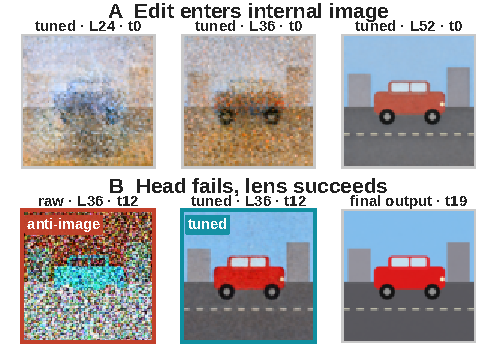
\includegraphics[width=0.98\columnwidth]{figs/fig12_tuned_lens/fig12_tuned_lens.pdf}
  \caption{\textbf{Internal image vs.\ frozen-head ghost.} \textbf{A}: the
  zero-shot tuned lens shows the edit enter a coherent internal image at
  $t{=}0$. \textbf{B}: for the same L36/$t$12 state, the frozen head yields
  an anti-image while the tuned lens recovers the edited scene.}
  \label{fig:tunedlens}
\end{figure}

\paragraph{The anti-image, mechanized.} This also explains a striking
artifact: the mid-stack \emph{frozen}-head decode at later steps is a
color-\emph{inverted} ghost (a cyan car under a red-brown sky) -- the
image-like mid-stack code forced through a head built to consume a
velocity, since $\hat x_0 = x_t - \sigma v$ flips the sign of an
image-like quantity. The tuned lens at the same cell is already coherent.
\noindent\textbf{Takeaway.} Mid-stack states are image-like; the L52--54 band
reconciles them to the velocity convention the head consumes.

\subsection{Transplantable, Writable, and Carrier-Bound}\label{sec:dissoc}

Reading a lens shows only that a representation is \emph{consistent with}
an edit, not what it can install. Whole-token ablation across many layers
drives the edited region off-manifold, so we use it only as a coarse stress
test rather than evidence for fine-grained necessity.

\paragraph{Transplant establishes sufficiency.} Transplanting a
\emph{car\_red} donor's car-region hidden states into a \emph{car\_green}
recipient (which alone scores $P(\text{red}){=}0.011$) flips the output to
red from \emph{any} of four donor bands, including \textbf{L48--59}
($0.940$). The donor representation is therefore sufficient to install
the edit. A content control confirms specificity: splicing the same
donor's \emph{background}-region tokens (right band, wrong content) yields
a garbled ``blue car'' ($0.991$), not red.

\paragraph{Readability does not imply unconstrained writability.} A single stored
\emph{direction} -- the probe's $d_{\text{red}}$, no donor pass -- added to
the recipient's car rows gives a sharp sigmoidal dose-response ($0.024$ at
$\alpha{=}0.5$, $0.977$ at $\alpha{=}1$, saturating to $\alpha{=}8$); a
random direction of equal norm is inert ($0.017$), and the negated
direction overshoots to blue ($0.945$), reproducing the anti-image under
an active intervention. But writability is bounded: at effective doses the
steered region is not a recolored car but a flat red patch that
\emph{replaces} the car's geometry -- the direction installs \emph{which}
hue, not \emph{where to stop}. Supplying that missing ``where'' with the
edited object's own silhouette mask turns every previously-failing dose
into a clean in-place recolor (Figure~\ref{fig:carrier}). And conjuring an
\emph{object} outruns any single direction: the
identity probe direction is inert (the read and write subspaces
differ), while a rank ladder over the donor$-$recipient difference
resolves identity coarse-to-fine -- category at rank 1, a coherent
instance by rank 4, donor-faithful by rank 64 ($2\%$ of the model
dimension). The read and write subspaces differ, and a writable attribute
still requires a spatial carrier.

\begin{figure}[t]
  \centering
  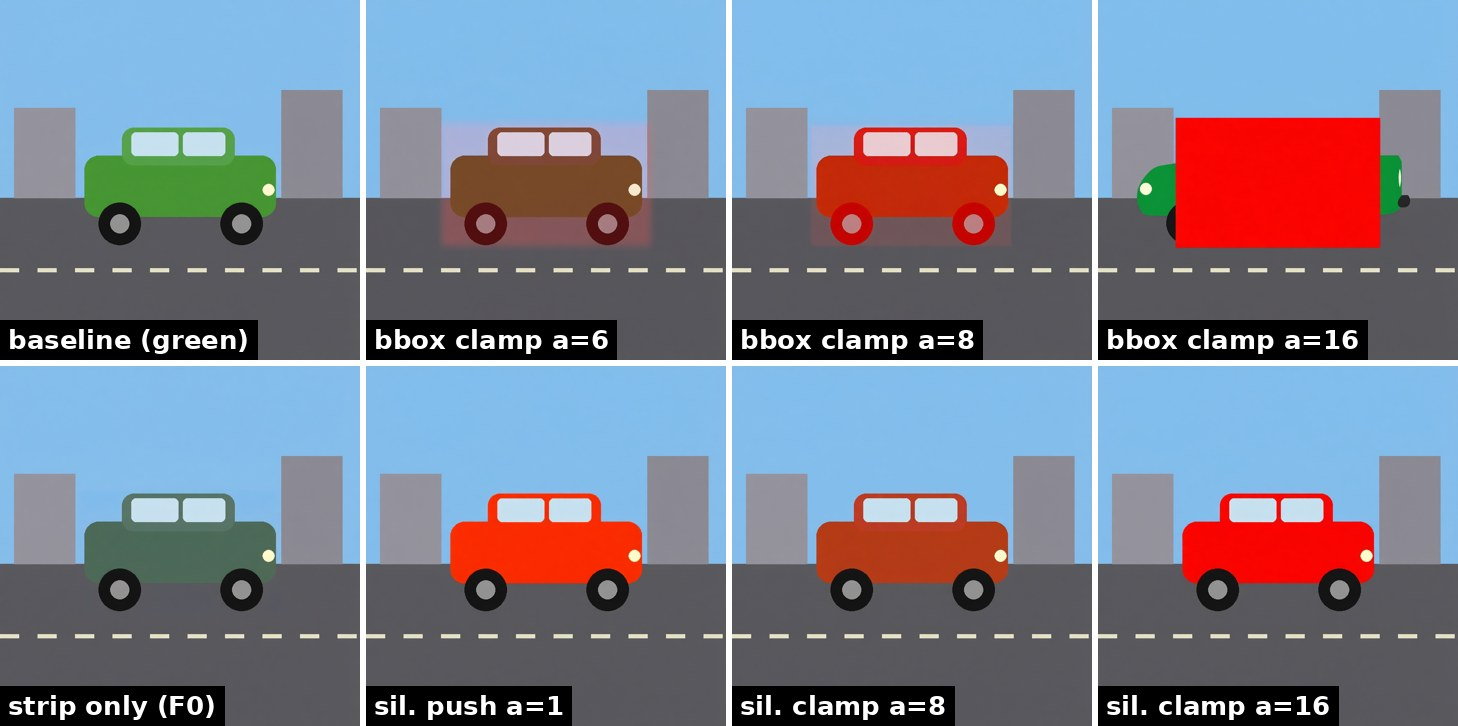
\includegraphics[width=0.48\columnwidth,viewport=0 363 364 726,clip]{figs/i1d_recompose_grid/i1d_recompose_grid.jpg}\hfill
  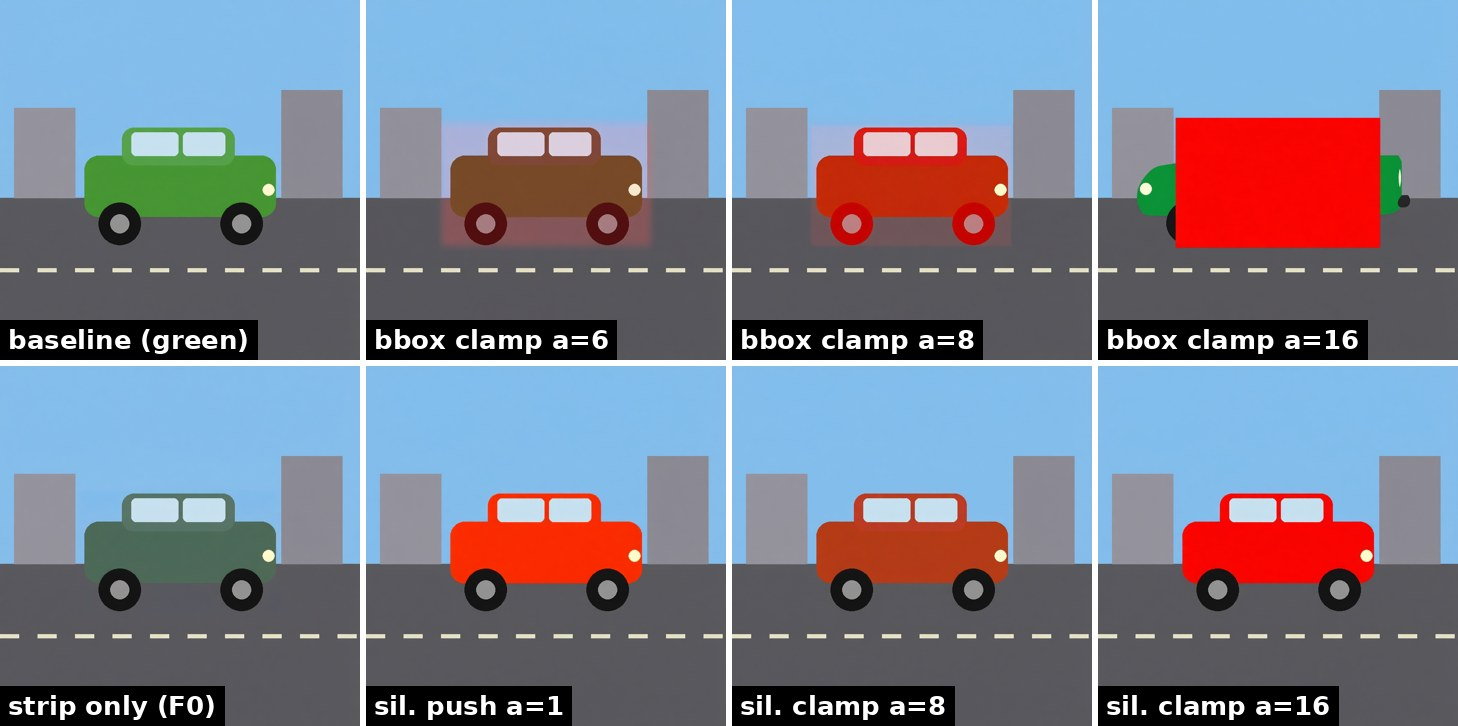
\includegraphics[width=0.48\columnwidth,viewport=1094 363 1458 726,clip]{figs/i1d_recompose_grid/i1d_recompose_grid.jpg}\\[-1pt]
  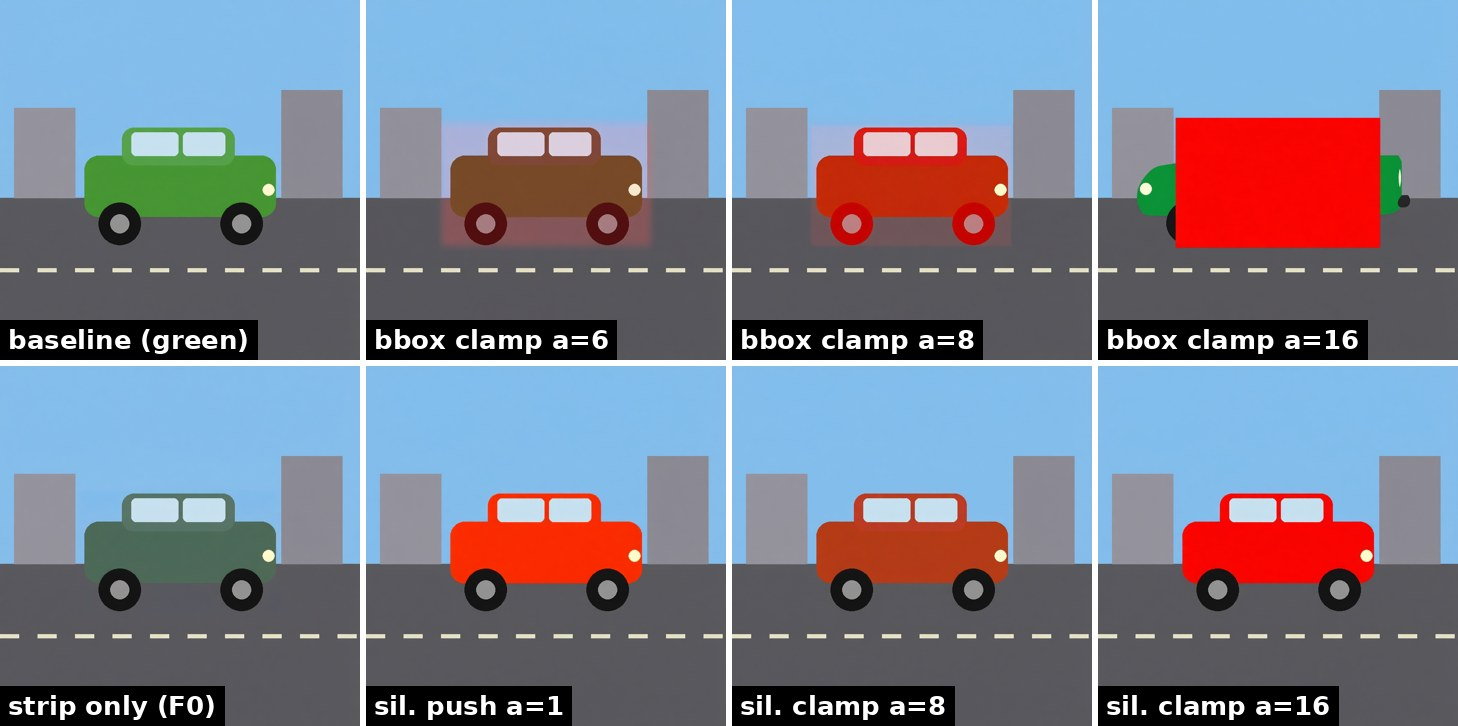
\includegraphics[width=0.48\columnwidth,viewport=729 0 1094 363,clip]{figs/i1d_recompose_grid/i1d_recompose_grid.jpg}\hfill
  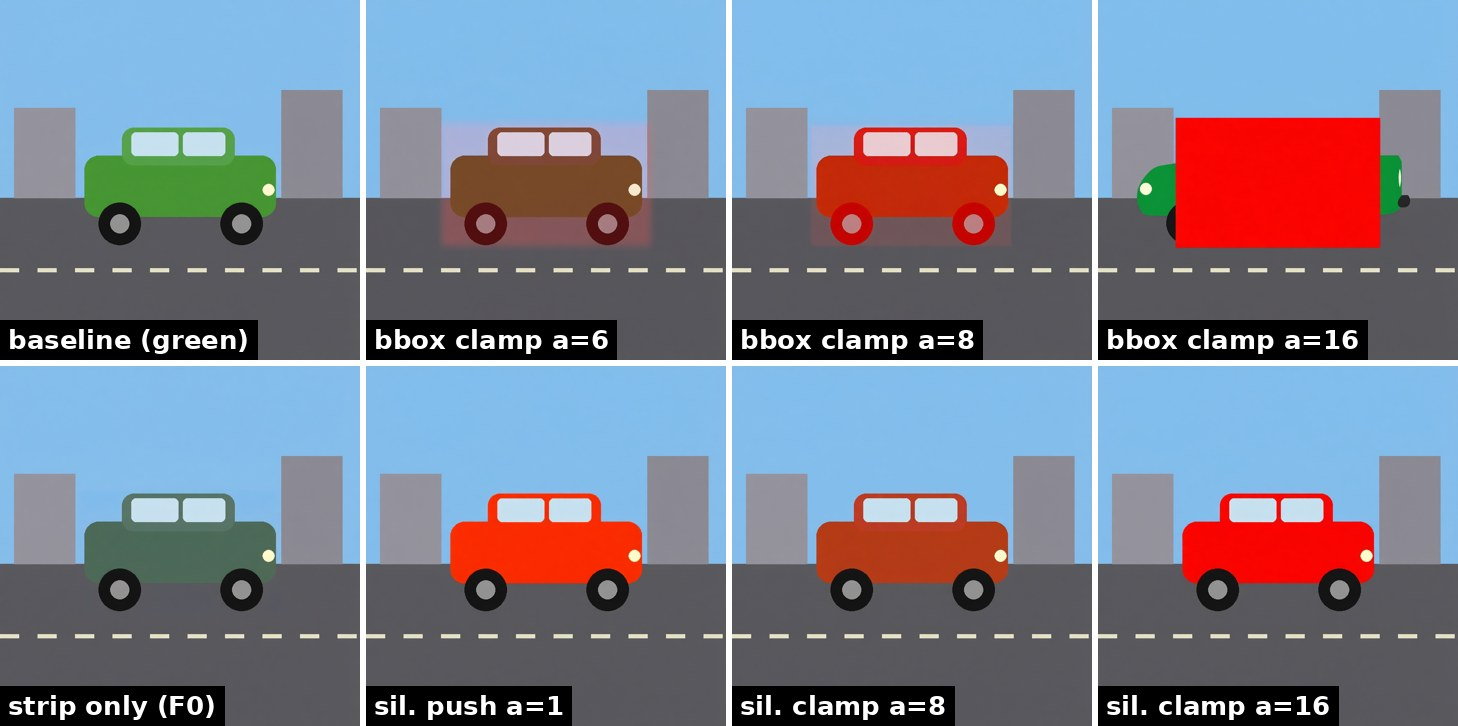
\includegraphics[width=0.48\columnwidth,viewport=1094 0 1458 363,clip]{figs/i1d_recompose_grid/i1d_recompose_grid.jpg}
  \caption{\textbf{A spatial carrier restores clean writability.}
  Steering red inside a bounding box eventually overwrites the car with a
  flat patch (top); the same direction restricted to the car silhouette
  preserves geometry across effective doses (bottom).}
  \label{fig:carrier}
\end{figure}

\subsection{A Preview Lever: The Differential Lens at 15\% NFE}\label{sec:difflens}

The differential lens (\emph{Proposed Method}) isolates the internal
edit plan from the reconstruction. It first settles a caveat left open
above: token-level $R^2$ \emph{inside} the edit region is
$0.88$--$0.97$, matching the full-image value, so the tuned
dictionaries carry the edit-specific signal itself, not incidental
scene detail.

\paragraph{Content is early; separation is gradual.} A pre-registered
prediction that $D$ would already localize tightly at every step is
refuted, informatively. The edit \emph{content} is present at step 0 (the
tuned lens already shows red eyes, a black trunk), but the
\emph{differential} at step 0 is a diffuse whole-frame field -- the edit
prompt perturbs the entire velocity relative to the no-op, not just the
edited region -- and condenses onto the edit's footprint only gradually
(localization of $D$'s top mass at L52 climbs monotonically across steps,
e.g.\ $0.21{\to}0.47{\to}0.67{\to}0.83$ for a cat's-eyes recolor).
\emph{Present} (content in the internal image) and \emph{separated}
(the differential has found where it lives) are different quantities.
The no-op control also caught one flat-art scene that \emph{cannot}
``do nothing'' (it renders a transparency checkerboard, and is
discarded), motivating the control-fidelity gate applied before any
differential number is trusted.

\paragraph{A preview lever.} Because the differential carries the edit's
footprint, we ask whether it does so early enough to be useful. At step 2
-- the third of 20, $\approx$15\% of the forward passes -- across a
10-case, five-family battery of natural photographs (all passing the
control-fidelity gate, $r\in[0.86,0.99]$), the median IoU between
$D_{\text{L52},t2}$'s top mass and a final-output difference mask is $0.33$,
$6.6\times$ chance, and all 10 cases sharpen from step 0 to step 2
(Figure~\ref{fig:preview}): an object slated for removal lights up as a
ghost, a keep-vs-replace background segmentation emerges unsupervised, and
a tiny recolor glows at its exact site. Because the no-op control is
\emph{independent of the edit prompt}, it is computed once per source
image and cached; previewing a \emph{candidate} edit then costs three
forward passes plus one frozen-dictionary decode, not a full 20-step run
-- a training-free way to triage many prompts against one image before
running any to completion.

\begin{figure}[t]
  \centering
  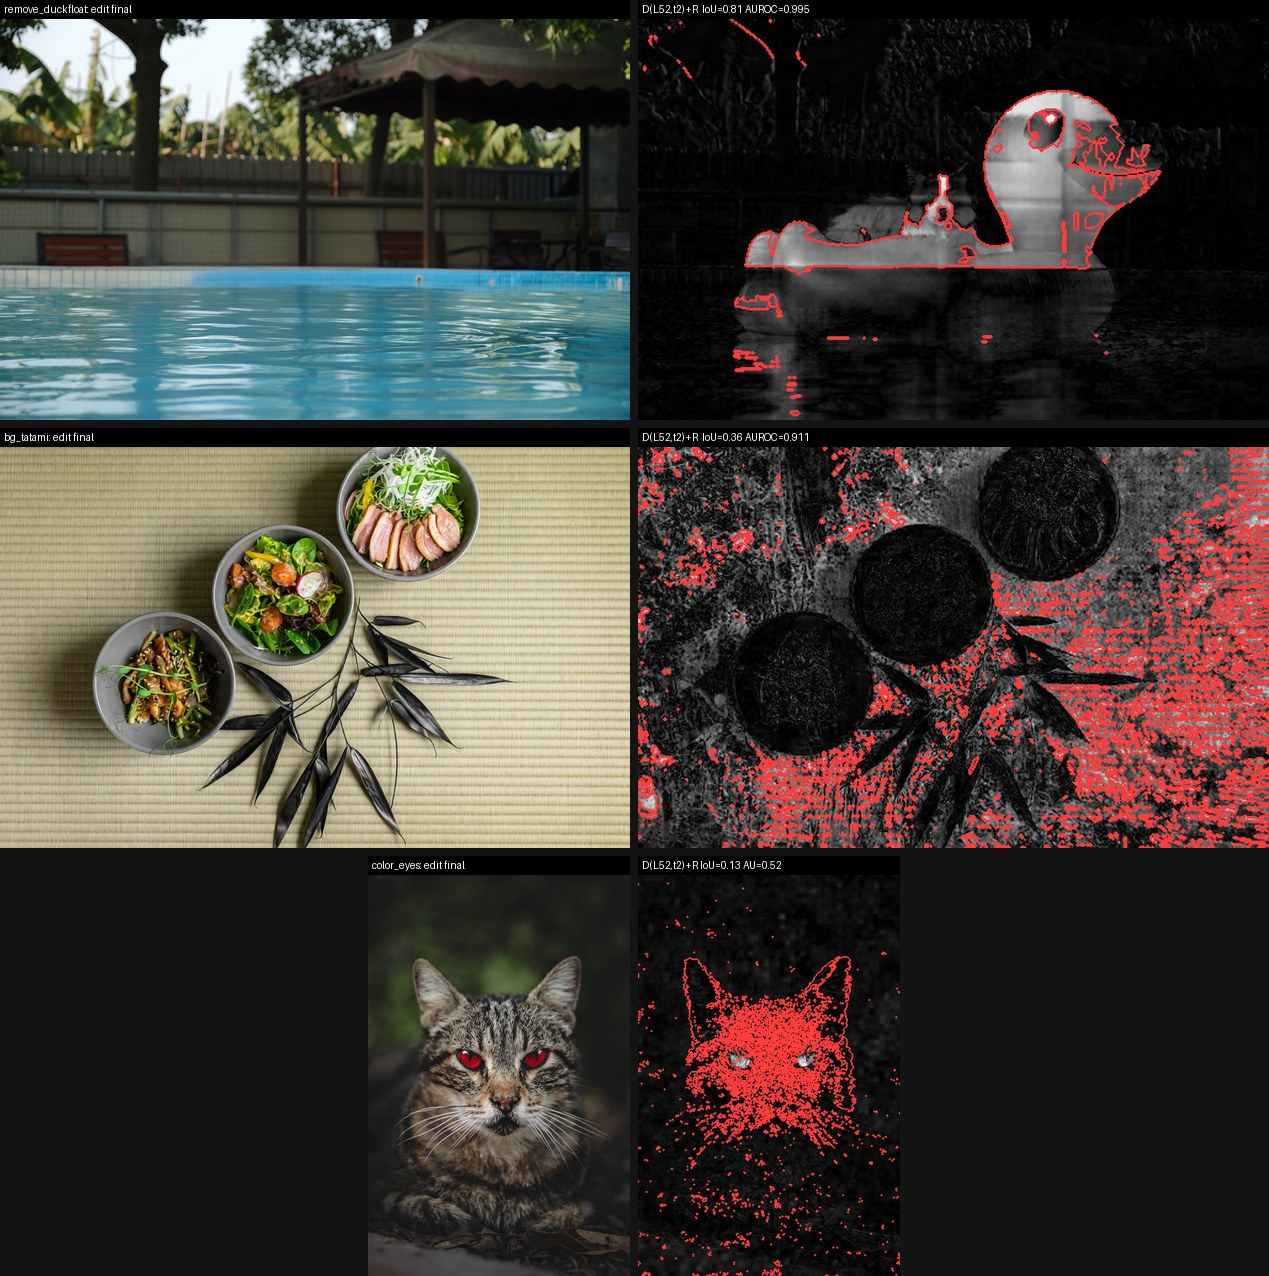
\includegraphics[width=\columnwidth]{figs/fig15_preview_lever/fig15_preview_lever.jpg}
  \caption{\textbf{Differential preview at 15\% NFE.} Final edits (left)
  and $D_{\mathrm{L52},t2}$ previews (right, final-output difference-mask
  boundary in red):
  removal, keep-vs-replace background structure, and a tiny recolor are
  visible after only three of twenty denoising steps.}
  \label{fig:preview}
\end{figure}

\subsection{Generalization Across Checkpoints}\label{sec:generalize}

Most mechanistic findings so far concern one model lineage. We re-ran the depth-lens
crossover and cross-seed probe on the two
further checkpoints from \emph{Setup} (FireRed-Image-Edit-1.1 and
Rapid-AIO). \textbf{The translation boundary and explicit-prompt early
readability replicate} (Table~\ref{tab:generalize}). FireRed has the same
flat-then-dip probe shape, and Rapid-AIO preserves the boundary under a
four-step schedule. The readable direction also transfers between Qwen and
FireRed, rather than merely recurring at the same layer index. The full tuned
lens ports to FireRed as well (deep-layer $R^2$ $0.97$--$0.999$; anti-image
reproduced).

\begin{table}[t]
\caption{Cross-checkpoint translation and early readout. Transfer is
Qwen$\to$FireRed / FireRed$\to$Qwen; L12/$t$4 direction cosine is .833.}
\label{tab:generalize}
\centering
\footnotesize
\setlength{\tabcolsep}{3pt}
\begin{tabular}{@{}lccc@{}}
\toprule
Checkpoint & A/C band & Probe: early $\to$ L59 & Transfer \\
\midrule
Qwen & L52--54 & .883 @ L6/$t$4 $\to$ .68--.70 & source \\
FireRed & L53--56 & .852 @ L6/$t$4 $\to$ .69--.70 & .840/.917 \\
Rapid-AIO & L52--54 & -- & -- \\
\bottomrule
\end{tabular}
\end{table}

\subsection{A Training-Free Lever: Truncating Classifier-Free Guidance}\label{sec:lever}

The layer--time map suggests a simple existence proof: classifier-free
guidance may not need both forward passes at all 20 steps. Running the unconditional pass
only for the first two steps and the conditional pass alone thereafter
leaves all four tested edit families visually intact at a \textbf{45\% reduction
in forward passes} (a 20-case battery confirms it, mean $1.77\times$
speedup). Dropping CFG entirely suggests where its non-redundant role lies in these cases: recolor, removal,
and addition still land from the conditional pass alone, but background
swap composites the new scene \emph{around} un-erased source structure
($P(\text{beach}){=}0.45$ vs.\ ${\ge}0.996$) -- CFG's non-redundant
contribution here is consistent with resolving \emph{scope}, not selecting edit content. The same
layer--time structure survives $7.7\times$ step distillation (20/20 cases
land), so distillation compresses the sampling trajectory but not the
structure the lens exposes.

\subsection{Limitations}\label{sec:limits}

Translation/intervention evidence uses Qwen plus two same-lineage checkpoints;
Boogu supports only outcome prediction/selection. The fixed-prompt probe has
one synthetic source; natural-image follow-ups give two replications and one
unsuitable eye case. Selection has 12 groups per task and cannot create absent
targets. One-way L6 hue transfer (mug$\to$tree $p{=}0.002$; reverse
$p{=}0.968$) precludes an object-invariant subspace. Because CLIP can prefer a
flat patch to a true recolor, quantitative claims carry pre-registered visual
verdicts. The dense boundary and carrier intervention both center on the
flat-art car; the carrier silhouette is derived from a source--edit pixel
difference rather than an automatic segmentation. The preview reference is a fixed top-10\% final-output difference
mask, which can over-expand tiny edits; its IoU is therefore a localization
diagnostic, not segmentation ground truth. We claim tested outcome predictability, transplant sufficiency, and
carrier-bounded writability, not irreversible commitment or necessity.
